
%% bare_conf.tex
%% V1.4b
%% 2015/08/26
%% by Michael Shell
%% See:
%% http://www.michaelshell.org/
%% for current contact information.
%%
%% This is a skeleton file demonstrating the use of IEEEtran.cls
%% (requires IEEEtran.cls version 1.8b or later) with an IEEE
%% conference paper.
%%
%% Support sites:
%% http://www.michaelshell.org/tex/ieeetran/
%% http://www.ctan.org/pkg/ieeetran
%% and
%% http://www.ieee.org/

%%*************************************************************************
%% Legal Notice:
%% This code is offered as-is without any warranty either expressed or
%% implied; without even the implied warranty of MERCHANTABILITY or
%% FITNESS FOR A PARTICULAR PURPOSE! 
%% User assumes all risk.
%% In no event shall the IEEE or any contributor to this code be liable for
%% any damages or losses, including, but not limited to, incidental,
%% consequential, or any other damages, resulting from the use or misuse
%% of any information contained here.
%%
%% All comments are the opinions of their respective authors and are not
%% necessarily endorsed by the IEEE.
%%
%% This work is distributed under the LaTeX Project Public License (LPPL)
%% ( http://www.latex-project.org/ ) version 1.3, and may be freely used,
%% distributed and modified. A copy of the LPPL, version 1.3, is included
%% in the base LaTeX documentation of all distributions of LaTeX released
%% 2003/12/01 or later.
%% Retain all contribution notices and credits.
%% ** Modified files should be clearly indicated as such, including  **
%% ** renaming them and changing author support contact information. **
%%*************************************************************************


% *** Authors should verify (and, if needed, correct) their LaTeX system  ***
% *** with the testflow diagnostic prior to trusting their LaTeX platform ***
% *** with production work. The IEEE's font choices and paper sizes can   ***
% *** trigger bugs that do not appear when using other class files.       ***                          ***
% The testflow support page is at:
% http://www.michaelshell.org/tex/testflow/



\documentclass[conference, spanish]{IEEEtran}
% Some Computer Society conferences also require the compsoc mode option,
% but others use the standard conference format.
%
% If IEEEtran.cls has not been installed into the LaTeX system files,
% manually specify the path to it like:
% \documentclass[conference]{../sty/IEEEtran}


\usepackage[spanish]{babel}
\usepackage[utf8]{inputenc}
\usepackage[T1]{fontenc}
\usepackage{caption}
\usepackage{graphicx}


\usepackage{listings}
\usepackage{color}
\usepackage{array}
\usepackage{colortbl}
\usepackage{xcolor}

\usepackage{float}
\usepackage{subfloat}
\usepackage{subfig}
\usepackage{pbox}



% Some very useful LaTeX packages include:
% (uncomment the ones you want to load)


% *** MISC UTILITY PACKAGES ***
%
%\usepackage{ifpdf}
% Heiko Oberdiek's ifpdf.sty is very useful if you need conditional
% compilation based on whether the output is pdf or dvi.
% usage:
% \ifpdf
%   % pdf code
% \else
%   % dvi code
% \fi
% The latest version of ifpdf.sty can be obtained from:
% http://www.ctan.org/pkg/ifpdf
% Also, note that IEEEtran.cls V1.7 and later provides a builtin
% \ifCLASSINFOpdf conditional that works the same way.
% When switching from latex to pdflatex and vice-versa, the compiler may
% have to be run twice to clear warning/error messages.






% *** CITATION PACKAGES ***
%
%\usepackage{cite}
% cite.sty was written by Donald Arseneau
% V1.6 and later of IEEEtran pre-defines the format of the cite.sty package
% \cite{} output to follow that of the IEEE. Loading the cite package will
% result in citation numbers being automatically sorted and properly
% "compressed/ranged". e.g., [1], [9], [2], [7], [5], [6] without using
% cite.sty will become [1], [2], [5]--[7], [9] using cite.sty. cite.sty's
% \cite will automatically add leading space, if needed. Use cite.sty's
% noadjust option (cite.sty V3.8 and later) if you want to turn this off
% such as if a citation ever needs to be enclosed in parenthesis.
% cite.sty is already installed on most LaTeX systems. Be sure and use
% version 5.0 (2009-03-20) and later if using hyperref.sty.
% The latest version can be obtained at:
% http://www.ctan.org/pkg/cite
% The documentation is contained in the cite.sty file itself.






% *** GRAPHICS RELATED PACKAGES ***
%
\ifCLASSINFOpdf
  % \usepackage[pdftex]{graphicx}
  % declare the path(s) where your graphic files are
  % \graphicspath{{../pdf/}{../jpeg/}}
  % and their extensions so you won't have to specify these with
  % every instance of \includegraphics
  % \DeclareGraphicsExtensions{.pdf,.jpeg,.png}
\else
  % or other class option (dvipsone, dvipdf, if not using dvips). graphicx
  % will default to the driver specified in the system graphics.cfg if no
  % driver is specified.
  % \usepackage[dvips]{graphicx}
  % declare the path(s) where your graphic files are
  % \graphicspath{{../eps/}}
  % and their extensions so you won't have to specify these with
  % every instance of \includegraphics
  % \DeclareGraphicsExtensions{.eps}
\fi
% graphicx was written by David Carlisle and Sebastian Rahtz. It is
% required if you want graphics, photos, etc. graphicx.sty is already
% installed on most LaTeX systems. The latest version and documentation
% can be obtained at: 
% http://www.ctan.org/pkg/graphicx
% Another good source of documentation is "Using Imported Graphics in
% LaTeX2e" by Keith Reckdahl which can be found at:
% http://www.ctan.org/pkg/epslatex
%
% latex, and pdflatex in dvi mode, support graphics in encapsulated
% postscript (.eps) format. pdflatex in pdf mode supports graphics
% in .pdf, .jpeg, .png and .mps (metapost) formats. Users should ensure
% that all non-photo figures use a vector format (.eps, .pdf, .mps) and
% not a bitmapped formats (.jpeg, .png). The IEEE frowns on bitmapped formats
% which can result in "jaggedy"/blurry rendering of lines and letters as
% well as large increases in file sizes.
%
% You can find documentation about the pdfTeX application at:
% http://www.tug.org/applications/pdftex





% *** MATH PACKAGES ***
%
%\usepackage{amsmath}
% A popular package from the American Mathematical Society that provides
% many useful and powerful commands for dealing with mathematics.
%
% Note that the amsmath package sets \interdisplaylinepenalty to 10000
% thus preventing page breaks from occurring within multiline equations. Use:
%\interdisplaylinepenalty=2500
% after loading amsmath to restore such page breaks as IEEEtran.cls normally
% does. amsmath.sty is already installed on most LaTeX systems. The latest
% version and documentation can be obtained at:
% http://www.ctan.org/pkg/amsmath





% *** SPECIALIZED LIST PACKAGES ***
%
%\usepackage{algorithmic}
% algorithmic.sty was written by Peter Williams and Rogerio Brito.
% This package provides an algorithmic environment fo describing algorithms.
% You can use the algorithmic environment in-text or within a figure
% environment to provide for a floating algorithm. Do NOT use the algorithm
% floating environment provided by algorithm.sty (by the same authors) or
% algorithm2e.sty (by Christophe Fiorio) as the IEEE does not use dedicated
% algorithm float types and packages that provide these will not provide
% correct IEEE style captions. The latest version and documentation of
% algorithmic.sty can be obtained at:
% http://www.ctan.org/pkg/algorithms
% Also of interest may be the (relatively newer and more customizable)
% algorithmicx.sty package by Szasz Janos:
% http://www.ctan.org/pkg/algorithmicx




% *** ALIGNMENT PACKAGES ***
%
%\usepackage{array}
% Frank Mittelbach's and David Carlisle's array.sty patches and improves
% the standard LaTeX2e array and tabular environments to provide better
% appearance and additional user controls. As the default LaTeX2e table
% generation code is lacking to the point of almost being broken with
% respect to the quality of the end results, all users are strongly
% advised to use an enhanced (at the very least that provided by array.sty)
% set of table tools. array.sty is already installed on most systems. The
% latest version and documentation can be obtained at:
% http://www.ctan.org/pkg/array


% IEEEtran contains the IEEEeqnarray family of commands that can be used to
% generate multiline equations as well as matrices, tables, etc., of high
% quality.




% *** SUBFIGURE PACKAGES ***
%\ifCLASSOPTIONcompsoc
%  \usepackage[caption=false,font=normalsize,labelfont=sf,textfont=sf]{subfig}
%\else
%  \usepackage[caption=false,font=footnotesize]{subfig}
%\fi
% subfig.sty, written by Steven Douglas Cochran, is the modern replacement
% for subfigure.sty, the latter of which is no longer maintained and is
% incompatible with some LaTeX packages including fixltx2e. However,
% subfig.sty requires and automatically loads Axel Sommerfeldt's caption.sty
% which will override IEEEtran.cls' handling of captions and this will result
% in non-IEEE style figure/table captions. To prevent this problem, be sure
% and invoke subfig.sty's "caption=false" package option (available since
% subfig.sty version 1.3, 2005/06/28) as this is will preserve IEEEtran.cls
% handling of captions.
% Note that the Computer Society format requires a larger sans serif font
% than the serif footnote size font used in traditional IEEE formatting
% and thus the need to invoke different subfig.sty package options depending
% on whether compsoc mode has been enabled.
%
% The latest version and documentation of subfig.sty can be obtained at:
% http://www.ctan.org/pkg/subfig




% *** FLOAT PACKAGES ***
%
%\usepackage{fixltx2e}
% fixltx2e, the successor to the earlier fix2col.sty, was written by
% Frank Mittelbach and David Carlisle. This package corrects a few problems
% in the LaTeX2e kernel, the most notable of which is that in current
% LaTeX2e releases, the ordering of single and double column floats is not
% guaranteed to be preserved. Thus, an unpatched LaTeX2e can allow a
% single column figure to be placed prior to an earlier double column
% figure.
% Be aware that LaTeX2e kernels dated 2015 and later have fixltx2e.sty's
% corrections already built into the system in which case a warning will
% be issued if an attempt is made to load fixltx2e.sty as it is no longer
% needed.
% The latest version and documentation can be found at:
% http://www.ctan.org/pkg/fixltx2e


%\usepackage{stfloats}
% stfloats.sty was written by Sigitas Tolusis. This package gives LaTeX2e
% the ability to do double column floats at the bottom of the page as well
% as the top. (e.g., "\begin{figure*}[!b]" is not normally possible in
% LaTeX2e). It also provides a command:
%\fnbelowfloat
% to enable the placement of footnotes below bottom floats (the standard
% LaTeX2e kernel puts them above bottom floats). This is an invasive package
% which rewrites many portions of the LaTeX2e float routines. It may not work
% with other packages that modify the LaTeX2e float routines. The latest
% version and documentation can be obtained at:
% http://www.ctan.org/pkg/stfloats
% Do not use the stfloats baselinefloat ability as the IEEE does not allow
% \baselineskip to stretch. Authors submitting work to the IEEE should note
% that the IEEE rarely uses double column equations and that authors should try
% to avoid such use. Do not be tempted to use the cuted.sty or midfloat.sty
% packages (also by Sigitas Tolusis) as the IEEE does not format its papers in
% such ways.
% Do not attempt to use stfloats with fixltx2e as they are incompatible.
% Instead, use Morten Hogholm'a dblfloatfix which combines the features
% of both fixltx2e and stfloats:
%
% \usepackage{dblfloatfix}
% The latest version can be found at:
% http://www.ctan.org/pkg/dblfloatfix




% *** PDF, URL AND HYPERLINK PACKAGES ***
%
%\usepackage{url}
% url.sty was written by Donald Arseneau. It provides better support for
% handling and breaking URLs. url.sty is already installed on most LaTeX
% systems. The latest version and documentation can be obtained at:
% http://www.ctan.org/pkg/url
% Basically, \url{my_url_here}.




% *** Do not adjust lengths that control margins, column widths, etc. ***
% *** Do not use packages that alter fonts (such as pslatex).         ***
% There should be no need to do such things with IEEEtran.cls V1.6 and later.
% (Unless specifically asked to do so by the journal or conference you plan
% to submit to, of course. )


% correct bad hyphenation here
\hyphenation{op-tical net-works semi-conduc-tor}



\begin{document}
%
% paper title
% Titles are generally capitalized except for words such as a, an, and, as,
% at, but, by, for, in, nor, of, on, or, the, to and up, which are usually
% not capitalized unless they are the first or last word of the title.
% Linebreaks \\ can be used within to get better formatting as desired.
% Do not put math or special symbols in the title.
\title{VirtShell\\Framework para aprovisionamiento de soluciones virtuales}


% author names and affiliations
% use a multiple column layout for up to three different
% affiliations
\author{\IEEEauthorblockN{Carlos Alberto Llano R.}
\IEEEauthorblockA{Escuela de Ingeniería de Sistemas y Computación\\
Universidad del Valle\\
Cali, Valle del Cauca\\
Email: carlos\_llano@hotmail.com}
\and
\IEEEauthorblockN{John Alexander Sanabria}
\IEEEauthorblockA{Escuela de Ingeniería de Sistemas y Computación\\
Universidad del Valle\\
Cali, Valle del Cauca\\
Email: john.sanabria@correounivalle.edu.co}}

% conference papers do not typically use \thanks and this command
% is locked out in conference mode. If really needed, such as for
% the acknowledgment of grants, issue a \IEEEoverridecommandlockouts
% after \documentclass

% for over three affiliations, or if they all won't fit within the width
% of the page, use this alternative format:
% 
%\author{\IEEEauthorblockN{Michael Shell\IEEEauthorrefmark{1},
%Homer Simpson\IEEEauthorrefmark{2},
%James Kirk\IEEEauthorrefmark{3}, 
%Montgomery Scott\IEEEauthorrefmark{3} and
%Eldon Tyrell\IEEEauthorrefmark{4}}
%\IEEEauthorblockA{\IEEEauthorrefmark{1}School of Electrical and Computer Engineering\\
%Georgia Institute of Technology,
%Atlanta, Georgia 30332--0250\\ Email: see http://www.michaelshell.org/contact.html}
%\IEEEauthorblockA{\IEEEauthorrefmark{2}Twentieth Century Fox, Springfield, USA\\
%Email: homer@thesimpsons.com}
%\IEEEauthorblockA{\IEEEauthorrefmark{3}Starfleet Academy, San Francisco, California 96678-2391\\
%Telephone: (800) 555--1212, Fax: (888) 555--1212}
%\IEEEauthorblockA{\IEEEauthorrefmark{4}Tyrell Inc., 123 Replicant Street, Los Angeles, California 90210--4321}}




% use for special paper notices
%\IEEEspecialpapernotice{(Invited Paper)}




% make the title area
\maketitle

% As a general rule, do not put math, special symbols or citations
% in the abstract
\begin{abstract}
En la actualidad, con la creciente adopción de modelos de computación como el \emph{Cloud Computing} \footnote{conocida también como servicios en la nube, es un paradigma que permite ofrecer servicios de computación a través de una red, que usualmente es Internet.} y el \emph{Grid Computing} \footnote{Un grid es un sistema de computación distribuido que permite coordinar computadoras de diferente hardware y software y cuyo fin es procesar una tarea que demanda una gran cantidad de recursos y poder de procesamiento.}, los ambientes computacionales se han tornado cada vez más sofisticados y complejos, requiriendo de soluciones que traten de manera integral el aprovisionamiento de diferentes servicios sobre ambientes virtuales capaces de atender la variable demanda computacional, a través del despliegue de infraestructuras elásticas de computación. Hoy en día, se encuentran diversas soluciones que abordan el problema de aprovisionamiento usando diferentes enfoques para el despliegue y orquestación de plataformas y servicios. Sin embargo, los enfoques actuales carecen de mecanismos de comunicación que permitan interoperar entre diferentes aplicaciones; En general, las soluciones actuales presentan dificultades para ser accedidas en una red, como internet y ejecutadas de manera remota. Este proyecto propone como objetivo principal, plantear el diseño de un framework orientado al web, cuyas partes permitan el eficiente aprovisionamiento de software de manera automática para ambientes virtualizados.\\
\end{abstract}

% no keywords




% For peer review papers, you can put extra information on the cover
% page as needed:
% \ifCLASSOPTIONpeerreview
% \begin{center} \bfseries EDICS Category: 3-BBND \end{center}
% \fi
%
% For peerreview papers, this IEEEtran command inserts a page break and
% creates the second title. It will be ignored for other modes.
\IEEEpeerreviewmaketitle



\section{Introducción}
La aparición de ambientes de computación centrados en la nube, los cuales se caracterizan por ofrecer servicios bajo demanda, ha favorecido el desarrollo de diversas herramientas que apoyan los procesos de aprovisionamiento en demanda de servicios y ambientes de computación orientados al procesamiento de tareas de larga duración y manejo de grandes volúmenes de datos. Estos ambientes dinámicos de computación son desarrollados mayormente a través de técnicas de programación ágil las cuales se caracterizan por ofrecer rápidos resultados e integración a gran escala de componentes de software. Es así como los equipos de DevOps \footnote{DevOps consiste en traer las prácticas del desarrollo ágil a la administración de sistema y el trabajo en conjunto entre desarrolladores y administradores de sistemas. DevOps no es una descripción de cargo o el uso de herramientas, sino un método de trabajo enfocado a resultados.} se convierten en un elemento fundamental ya que potencia la estabilidad y uniformidad de los distintos ambientes de prueba y producción de modo que los procesos de integración y despliegue se hagan de forma automatizada. \\
\\
Las herramientas de aprovisionamiento automático de infraestructura son el eje central de estos equipos ya que es a través de ellas que el personal de desarrollo y operaciones son capaces de hablar un mismo lenguaje y establecer los requerimientos y necesidades a satisfacer. Sin embargo, las herramientas actuales de aprovisionamiento adolecen de servicios que faciliten la especificación de infraestructura a través de un API \footnote{ API: Application Programming Interface, conjunto de subrutinas, funciones y procedimientos que ofrece un software para ser utilizado por otro software como una capa de abstracción.} estandarizado que posibilite la orquestación del despliegue de infraestructura a través de Internet.\\
\\
En este artículo se presenta una herramienta de aprovisionamiento con orientación a servicios que permite el despliegue y orquestación de plataformas y servicios a través de un API RESTful \footnote{RESTful hace referencia a un servicio web que implementa la arquitectura REST}. Además de lo mencionado anteriormente, la artículo consta de 3 secciones.\\
\\
La segunda sección introduce y elabora la arquitectura planteada en VirtShell. Se describe los requisitos que se tuvieron en cuenta para elaborar la estructura del framework, las alternativas estudiadas y las características que conforman a VirtShell.\\
\\
Las tercera sección se encargan de describir cada uno de los módulos diseñados, ilustrando sus funcionalidades y la forma en que interactúan de manera conjunta para administrar la infraestructura y realizar el aprovisionamiento de los recursos virtualizados.\\
\\
En la cuarta sección se indican los métodos HTTP con que cuenta cada módulo que permiten interactuar con el API.\\
\\
Finalmente, la ultima sección se presentan las conclusiones.


\section{Arquitectura}
VirtShell Framework es concebido como una plataforma que proporciona herramientas para la automatización y gestión de infraestructura, facilitando tareas como la creación, despliegue, mantenimiento y monitoreo tanto de recursos virtuales como físicos vía web. Así mismo, es pensada para que cualquier desarrollo de software con acceso a Internet (sitio web, aplicación móvil, etc.) pueda interactuar con la infraestructura virtual tan solo consumiendo un API de Internet.\\
\\
Las motivaciones mencionadas conducen a los requisitos para una arquitectura destinada a separar claramente responsabilidades, usando protocolos abiertos, modificables, escalables, y al mismo tiempo adecuado para la creación rápida de nuevas acciones. \\
\\
En la búsqueda del adecuado estilo arquitectural para el API de VirtShell, se evaluaron dos estilos de servicios web: el estilo \emph{Remote Procedure Call} (RPC) y el estilo arquitectural REST (\emph{Representational State Transfer}) \cite{fielding00}. La evaluación dio como resultado que el estilo arquitectural que mejor se acomodaba a los requisitos planteados era el estilo arquitectural REST, debido a que es un estilo nativo del Web, lo que hace que la información disponible esta regida por las mismas normas que rigen los sitios web, ademas, el estilo ofrece mejor escalabilidad, acoplamiento y rendimiento. Un detallado comparativo entre los dos estilos se encuentra en \cite{Xinyang09}. 

\subsection{Características}
VirtShell es un framework de código abierto y bajo la licencia BSD, que permite utilizarlo para proyectos de cualquier tipo, incluso comerciales, sus características principales son: 

\begin{itemize}
\item \emph{Programable}: VirtShell esta orientado a realizar el aprovisionamiento de sus instancias principalmente por medio de scripts escritos en shell, permitiendo aprovechar todas las estructuras y utilidades del lenguaje de programación. Sin embargo, el lenguaje de shell no es de uso obligatorio, el  método de aprovisionamiento puede ser el de la preferencia del usuario. 
\item \emph{Repetible}: VirtShell ofrece herramientas para que los scritps de aprovisionamiento sean configurables y  puedan ser ejecutados varias veces en diferentes ambientes de desarrollo o producción.
\item \emph{Modular}: VirtShell es un framework organizado de forma modular. Los módulos se encuentran agrupados en categorías que ofrecen las herramientas necesarias para la administración y aprovisionamiento de múltiples recursos virtuales. De igual manera y dada las características de REST, los módulos están diseñados para que se puedan dividir en diferentes servidores obteniendo "micro APIs", lo que permite dividir los procesos y atender diferentes tipos de operaciones del API. 
\item \emph{Seguro}: VirtShell provee varias capacidades y servicios para aumentar la privacidad y el control de acceso a los diferentes recursos. Los servicios de seguridad permiten crear redes y controlar el acceso a las instancias creadas, así como definir y administrar políticas de acceso a usuarios y permisos sobre cualquier recurso del sistema como por ejemplo scripts de creación y aprovisionamiento.
\item \emph{Extensible}: Al ser VirtShell de código abierto, el API puede modificarse, crecer fácilmente y versionarse de diferentes maneras. Adicionalmente, VirtShell fue diseñado con la idea de cargar código dinámicamente, permitiendo extender el comportamiento del framework agregando plugins en tiempo de ejecución.  Asi mismo, VirtShell permite extender el comportamiento del shell desplegando comandos propios que proporcionan ahorro en tiempo y en complejidad.
\item \emph{Inyección de dependencias virtuales}: VirtShell adopta la idea del patrón de Inyección de Dependencias \footnote{es un patrón de diseño orientado a objetos, en el que se suministran objetos a una clase en lugar de ser la propia clase quien cree el objeto. El término fue acuñado por primera vez por Martin Fowler.} \cite{fowler04} para conseguir scripts de aprovisionamiento mas desacoplados. De esta manera facilita la configuración de las dependencias que tiene un recurso virtual de otras máquinas virtuales. Para ello, el framework permite declarar el listado de dependencias de recursos virtuales que tiene un script de aprovisionamiento encargándose del correcto acople entre los diferentes recursos virtuales.
\item \emph{Interoperable}: Al seguir el estilo arquitectónico REST y contar con la documentación detallada sobre cada uno de los recursos y urls que expone el API de VirtShell, se logra una capacidad clave para la administración remota de la infraestructura virtual. Esta capacidad se refiere al hecho de poder desarrollar aplicaciones en cualquier plataforma y para cualquier dispositivo electrónico, lo que permite funcionar con otros productos o sistemas existentes o futuros.

\end{itemize}

\section{Módulos}
VirtShell Framework consiste de características organizadas en 13 módulos. Estos módulos son agrupados en Seguridad, Administración y Aprovisionamiento. Estos elementos se usan de manera separada pero trabajan juntos para proveer la información necesaria para que los agentes realicen su trabajo en los hosts que albergaran los recursos virtuales, como se muestra en la figura \ref{fig:framework}. \\

\begin{figure}[h]
  \centering
  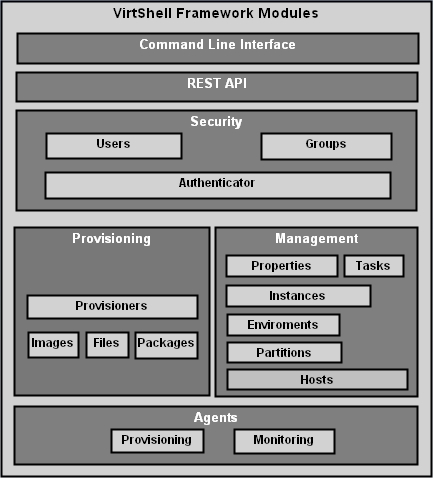
\includegraphics[width = 0.4\textwidth]{../architecture/v1/diagrams/framework}
  \caption{Visión general del framework de VirtShell}
  \label{fig:framework}
\end{figure}

Las siguientes secciones detallan los módulos disponibles para cada característica. 

\subsection{Security}
Seguridad consiste de los módulos de \emph{users} (usuarios), \emph{groups} (grupos) y el modulo \emph{authenticator} (de autenticación). El control de los usuarios y grupos son elementos clave en la administración del framework. Los \textbf{Usuarios} pueden ser personas reales, es decir, cuentas ligadas a un usuario físico en particular o cuentas que existen para ser usadas por aplicaciones específicas. \\
\\
Los \textbf{Grupos} son expresiones lógicas de organización, reuniendo usuarios para un propósito común. Los usuarios dentro de un mismo grupo pueden leer, escribir o ejecutar los recursos que pertenecen a ese grupo.\\
\\
El módulo de \textbf{autenticación} soporta el proceso por el cual cuando un usuario se presenta a la aplicación puede validar su identidad. Este módulo es quien decide0 si el usuario tiene permiso para ingresar al sistema y el nivel de acceso a un recurso dado. En el capitulo 4 se detalla el proceso de autenticación y autorización.

\subsection{Managment}
Administración consiste de los modulos \emph{hosts} (anfitriónes), \emph{partitions} (particiones), \emph{enviroments} (ambientes), \emph{instances} (instancias), \emph{properties} (propiedades) y \emph{tasks} (tareas). \\
\\
El módulo de \textbf{anfitriónes} lleva registro de nodos físicos, servidores o máquinas virtuales, que se encuentren conectados a la red y que permitan albergar instancias virtuales. Los anfitriónes son clasificados de acuerdo a diferentes combinaciones de CPU, memoria, almacenamiento y capacidad de trabajo en red, dando flexibilidad para elegir la opcion mas adecuada para las necesidades de las aplicaciones destino. En otras palabras el tipo de anfitrión determina el hardware del nodo físico que sera usado por los recursos virtuales.\\
\\
El módulo de \textbf{particiones} permite dividir los anfitriones en secciones aisladas de disponibilidad. Cada partición puede ser usada para definir áreas geográficas separadas o simplemente para dividir los nodos físicos en subgrupos destinados a diferentes usos o equipos de trabajo o tipos de clientes.\\
\\
El módulo de \textbf{ambientes} permite dividir lógicamente una partición en subredes de trabajo más pequeñas, con lo que se crean grupos más pequeños con diferentes fines. En los ambientes de trabajo se configuran los usuarios que tienen permiso para interactuar trabajar con el.\\
\\
El módulo de \textbf{instancias} es un recurso virtual o máquina virtual o contenedor con parámetros y capacidades definidas en la cual se puede instalar el software deseado. Un usuario puede crear, aprovisionar, actualizar y finalizar instancias en VirtShell tanto como necesite dando la sensación de elasticidad \footnote{La elasticidad es una de las propiedades fundamentales de la nube. La elasticidad consiste en la potencia de escalar los recursos informáticos ampliándolos y reduciéndolos dinámicamente.} de la red.\\
\\
El módulo de \textbf{propiedades} permite consultar información de sistema, de las instancias o de los anfitriones físicos. La información que puede ser consultada es toda aquella que el sistema tenga disponible o que se pueda consultar por medio de comandos de sistema o comandos propios de VirtShell. Ejemplos de información que se puede consultar por medio de las propiedades es porcentajes de memoria y cpu usada, numero de procesos en ejecución, etc. Las propiedades pueden ser consultadas en una sola maquina, o simultáneamente en varias maquinas, o a un conjunto de maquinas de acuerdo a prefijos en su nombre.\\
\\
Finalmente, el módulo de \textbf{tareas} da la información y estado sobre las diferentes tareas o trabajos ejecutados en el sistema. Debido a que el medio para interactuar con los módulos de VirtShell es a través de un API REST, una petición de creación de un nuevo recurso virtual, puede ser largo si el aprovisionamiento involucra varias maquinas. Para evitar, tener una petición esperando respuesta, VirtShell crea una tarea que sera ejecutada de manera asincrónica, dando como respuesta, un identificador de la tarea, para que esta pueda ser consultada posteriormente y conocer el estado de la petición.


\subsection{Provisioning}
Aprovisionamiento consiste de los módulos \emph{provisioners} (aprovisonadores), \emph{images} (imágenes), \emph{files} (archivos) y \emph{packages} (paquetes).\\
\\
El módulo de \textbf{aprovisionadores} define un marco de aprovisionamiento de un recurso virtual y contiene las configuraciones necesarias para apoyar ese marco. La configuración fundamental de un aprovisionador, es la ruta del repositorio git \footnote{git es un software de control de versiones diseñado por Linus Torvalds}, donde se encuentran los scripts y archivos necesarios para realizar el aprovisionamiento. Del mismo modo la forma de ejecutar los scripts, hace parte de la configuración básica. Para ser mas ligero a VirtShell, los scripts de aprovisionamiento, deben estar registrados en un repositorio git público. VirtShell se encarga de descargar el repositorio y de ejecutar los scripts de aprovisionamiento, de acuerdo a la configuración especificada. \\
\\
Adicionalmente, los aprovisonadores cuentan con una manera de especificar las dependencias del nuevo recurso virtual. VirtShell se encarga de resolver las dependencias antes de realizar el aprovisionamiento del nuevo recurso, a su vez, suministra información de ellas a los scripts de aprovisionamiento si estos lo requieren. \\
\\
VirtShell utiliza como lenguaje de referencia, para la creación de scripts de aprovisionamiento, el lenguaje shell. Este cuenta con los recursos suficientes para interactuar con los diferentes sistemas operativos de las instancias. Sin embargo estos comandos se pueden extender usando el paquete de comandos propios de VirtShell, los cuales pueden abstraer muchas de las operaciones del shell. Esto facilita la escritura de los mismos o permite hacerlos independientes del sistema operativo en el cual van a ejecutarse.\\
\\
El módulo de \textbf{imágenes} proporciona la información necesaria de las imágenes que se encuentran registradas en el sistema. Cada vez que se crea un nuevo recurso virtual en un anfitrión, se especifica el nombre de la imagen almacenada en el sistema que sera usada, de una de las que se encuentra en el sistema. \\
\\
Las imágenes que se manejan en VirtShell son de dos tipos: ISO \footnote{Una imagen ISO es un archivo informático donde se almacena una copia o imagen exacta de un sistema de archivos o ficheros de un disco óptico, normalmente un disco compacto (CD) o un disco versátil digital (DVD).} y para contenedores. Las de tipo ISO, se encuentran guardadas en el repositorio de VirtShell, y su uso se enfoca a maquinas virtuales que interactuan con hypervisors. Las imágenes de tipo contenedor, se emplean para tecnologías de visualización de sistema operativo como LXC \footnote{LXC (Linux Containers) es una tecnología de virtualización a nivel de sistema operativo (SO) para Linux. } \cite{lxc16} y Docker \footnote{Docker es un proyecto de código abierto que automatiza el despliegue de aplicaciones dentro de contenedores de software, proporcionando una capa adicional de abstracción y automatización de Virtualización a nivel de sistema operativo en Linux.} \cite{docker16}. Estas son descargadas automáticamente de los repositorios de dominio público de los diferentes proveedores. \\
\\
El módulo de imágenes cuenta también, con la característica de crear automáticamente nuevas imágenes de tipo ISO a partir de las \emph{releases} (liberaciones) base de las diferentes distribuciones de sistemas operativos linux. Una vez creada la nueva ISO esta sera guardada en el repositorio interno para su posterior uso.\\
\\
El módulo de \textbf{archivos} proporciona una manera de almacenar archivos en VirtShell, los cuales pueden ser usados para almacenar 

El módulo de \textbf{archivos} proporciona una manera de almacenar archivos en VirtShell, los cuales pueden ser usados para almacenar información necesaria para crear imágenes o para enviarlos a uno o mas recursos virtuales de manera simultánea en un directorio especificado. Adicionalmente, permite especificar los permisos que tendrán los archivos.\\
\\
El módulo de \textbf{paquetes} facilita realizar funciones tales como la instalación de nuevos paquetes de software y actualización de paquetes existentes en uno o mas recursos virtuales de manera simultanea.


\subsection{Agents}
Los Agentes son servicios que se ejecutan localmente en cada anfitrión, y que se encuentra bajo la gestión de VirtShell. Estos son instalados y configurados en cada anfitrión de manera automática. Los agentes actúan con un cierto grado de autonomía con el fin de completar tareas en nombre del servidor.\\

\section{API}
API significa ``Application Programming Interface", y como término, especifica cómo debe interactuar el software.\\
\\
En términos generales, cuando nos referimos a las API de hoy, nos referimos más concretamente a las API web, que son manejadas a través del protocolo de transferencia de hipertexto (HTTP). Para este caso específico, entonces, una API especifica cómo un consumidor puede consumir el servicio que el API expone: cuales URI están disponibles, qué métodos HTTP puede utilizarse con cada URI, que parámetros de consulta se acepta, lo que los datos que pueden ser enviados en el cuerpo de la petición, y lo que el consumidor puede esperar como respuesta.\\
\\
En el VirtShell API REST un usuario enviá una solicitud al servidor para realizar una acción determinada (como la creación, recuperación, actualización o eliminación de un recurso virtual), y el servidor realiza la acción y enviá una respuesta, a menudo en la forma de una representación del recurso especificado.\\
\\
En el VirtShell API, el usuario especifica una acción con un verbo HTTP como POST, GET, PUT o DELETE. Especificando un recurso por un URI único global de la siguiente forma: \\
\\
\emph{https://[host]:[port]/virtshell/api/v1/resourcePath?parameters}\\
\\
Debido a que todos los recursos del API tienen una única URI HTTP accesible, REST permite el almacenamiento en cache de datos y esta optimizado para trabajar con una infraestructura distribuida de la web.\\
\\
En esta sección se detalla los recursos y operaciones que puede realizar un usuario del API para realizar aprovisionamientos automáticos desde cualquier plataforma de desarrollo. El VirtShell API provee acceso a los objetos en el VirtShell Server, esto incluye los hosts, imágenes, archivos, templates, aprovisionadores, instancias, grupos y usuarios. Por medio del API podrá crear ambientes, maquinas virtuales y contenedores personalizados, realizar configuraciones y administrar los recursos físicos y virtuales de manera programática. \\

\subsection{Formato de entrada y salida}
JSON (JavaScript Object Notation) es un formato de datos común, independiente del lenguaje que proporciona una representación de texto simple de estructuras de datos arbitrarias. Para obtener mas información, ver json.org.\\
\\
El VirtShell API solo soporta el formato json para intercambio de información. Cualquier solicitud que no se encuentre en formato json resultara en un error con código 406 (Content Not Acceptable Error).\\
\\
Las siguientes secciones muestran los métodos disponibles para cada módulo.\\

\subsection{Groups}
Representan los grupos registrados en VirtShell. Los métodos soportados son:

\begin{center}
 \captionof{table}{Métodos HTTP para groups}
 \small
 \begin{tabular}{| l | l | l |}
 \hline
  \textbf{Método} & \textbf{Solicitud} & \textbf{Descripción} \\ [0.5ex] 
  \hline\hline
  GET & /groups/:name & Gets one group by ID. \\
  \hline
  GET & /groups & Gets the list of groups. \\  
  \hline
  POST & /groups/ & creates a new group. \\
  \hline
  DELETE & /groups/:name & Deletes an existing group. \\
  \hline
\end{tabular}
\end{center}

\subsection{Users}
Representan los usuarios registrados en VirtShell. Los métodos soportados son:

\begin{center}
 \captionof{table}{Métodos HTTP para users}
 \small
 \begin{tabular}{| l | l | l |}
 \hline
  \textbf{Método} & \textbf{Solicitud} & \textbf{Descripción} \\ [0.5ex] 
  \hline\hline
  GET & /users/:name & Gets one user by ID. \\
  \hline
  POST & /users/ & creates a new user. \\
  \hline
  GET & /users & Gets the list of users. \\  
  \hline
  DELETE & /users/:name & Deletes an existing user. \\
  \hline  
  PUT & /users/:name & Updates an existing user. \\ [1ex]  
  \hline
\end{tabular}
\end{center}

\subsection{Partitions}
Las particones permiten organizar las máquinas que albergaran recursos virtuales en partes aisladas de las demás. Los métodos soportados son:

\begin{center}
 \captionof{table}{Métodos HTTP para partitions}
 \small
 \begin{tabular}{| l | l | l |}
 \hline
  \textbf{Método} & \textbf{Solicitud} & \textbf{Descripción} \\ [0.5ex] 
  \hline\hline
  GET & /partitions/:name & Gets one partition. \\
  \hline
  GET & /partitions & Gets the list of partitions. \\
  \hline  
  POST & /partitions/ & Inserts a new partition. \\
  \hline
  DELETE & /partitions/:name & Deletes apartition. \\
  \hline  
  PUT & \pbox{5cm}{/partitions/:name/ \\host/:hostname} & Add a host to partition. \\ [1ex] 
  \hline
\end{tabular}
\end{center}

\subsection{Hosts}
Representan las maquinas físicas; un host es un anfitrión de maquinas virtuales o contenedores. Los métodos soportados son:

\begin{center}
 \captionof{table}{Métodos HTTP para hosts}
 \small
 \begin{tabular}{| l | l | l |}
 \hline
 \textbf{Método} & \textbf{Solicitud} & \textbf{Descripción} \\ [0.5ex] 
  \hline\hline
  GET & /hosts/:name & Gets one host by name. \\
  \hline
  GET & /hosts & Gets the list of hosts. \\
  \hline  
  POST & /hosts/ & Inserts a new host. \\
  \hline
  DELETE & /hosts/:name & Deletes an existing host. \\
  \hline  
  PUT & /hosts/:name & Updates an existing host. \\ [1ex] 
  \hline
\end{tabular}
\end{center}


\subsection{Instances}
Representan las instancias de las máquinas virtuales o los contenedores. Los métodos soportados son:

\begin{center}
 \captionof{table}{Métodos HTTP para instances}
 \small
 \begin{tabular}{| l | l | l |}
 \hline
  \textbf{Método} & \textbf{Solicitud} & \textbf{Descripción} \\ [0.5ex] 
  \hline\hline
  GET & /provisioners/:name & Gets one provisioner by ID. \\
  \hline
  GET & /provisioners & Gets the list of provisioners. \\
  \hline  
  POST & /provisioners/ & Creates a new provisioner. \\
  \hline
  DELETE & /provisioners/:name & Deletes an existing host. \\ [1ex] 
  \hline
\end{tabular}
\end{center}


\subsection{Tasks}
Representan una tarea en VirtShell. Los métodos soportados son:

\begin{center}
 \captionof{table}{Métodos HTTP para tasks}
 \small
 \begin{tabular}{| l | l | l |}
 \hline
  \textbf{Método} & \textbf{Solicitud} & \textbf{Descripción} \\ [0.5ex] 
  \hline\hline
  GET & /tasks/:id & Gets one task by ID. \\
  \hline
  GET & /tasks & Gets the list of tasks. \\
  \hline
  GET & /tasks/status & Gets all task by status. \\
  \hline 
  POST & /tasks/ & Creates a new task \\
  \hline  
  PUT & /tasks/:id & Updates an existing task. \\ [1ex] 
  \hline
\end{tabular}
\end{center}

\subsection{Properties}
Representan propiedades de configuracián de las máquinas virtuales o contenedores. Los métodos soportados son:

\begin{center}
 \captionof{table}{Métodos HTTP para properties}
 \begin{tabular}{| l | l | l |}
 \hline
  \textbf{Método} & \textbf{Solicitud} & \textbf{Descripción} \\ [0.5ex] 
  \hline\hline
  GET & /properties/ & Install one or more packages. \\ [1ex] 
  \hline
\end{tabular}
\end{center}


\subsection{Provisioners}
Representan los scripts que aprovisionan las máquinas virtuales o los contenedores. Los métodos soportados son:

\begin{center}
 \captionof{table}{Métodos HTTP para provisioners}
 \begin{tabular}{| l | l | l |}
 \hline
  \textbf{Método} & \textbf{Solicitud} & \textbf{Descripción} \\ [0.5ex] 
  \hline\hline
  GET & /provisioners/:name & Gets one provisioner by ID. \\
  \hline
  GET & /provisioners & Gets the list of provisioners. \\
  \hline  
  POST & /provisioners/ & Creates a new provisioner. \\
  \hline
  DELETE & /provisioners/:name & Deletes an provisioner. \\
  \hline  
  PUT & /provisioners/:name & Updates a provisioner. \\ [1ex] 
  \hline
\end{tabular}
\end{center}

\subsection{Images}
Representan imagenes de máquinas virtuales o contenedores. Los métodos soportados son:

\begin{center}
 \captionof{table}{Métodos HTTP para images}
 \begin{tabular}{| l | l | l |}
 \hline
  \textbf{Método} & \textbf{Solicitud} & \textbf{Descripción} \\ [0.5ex] 
  \hline\hline
  GET & /images/:name & Gets one image by name. \\
  \hline
  GET & /images & Retrieves the list of images. \\
  \hline  
  POST & /images/ & Inserts a new image. \\
  \hline
  DELETE & /images/:name & Deletes an existing image. \\ [1ex] 
  \hline
\end{tabular}
\end{center}


\subsection{Packages}
Representan paquetes de software que se ejecutan en las máquinas virtuales o contenedores. Los métodos soportados son:

\begin{center}
 \captionof{table}{Métodos HTTP para packages}
 \begin{tabular}{| l | l | l |}
 \hline
  \textbf{Método} & \textbf{Solicitud} & \textbf{Descripción} \\ [0.5ex] 
  \hline\hline
  POST & /install\_packages/ & \pbox{4cm}{Install one or more\\ packages.} \\ 
  \hline
  POST & /upgrade\_packages/ & \pbox{4cm}{Upgrade one or more\\ packages.} \\
  \hline
  POST & /remove\_packages/ & \pbox{4cm}{Remove one or more \\packages.} \\ [1ex] 
  \hline
\end{tabular}
\end{center}

\subsection{Files}
Representan toda clase de archivos que se requieran para crear o aprovisionar máquinas virtuales o contenedores. Los métodos soportados son:

\begin{center}
\captionof{table}{Métodos HTTP para files}
 \begin{tabular}{| l | l | l |}
 \hline
  \textbf{Método} & \textbf{Solicitud} & \textbf{Descripción} \\ [0.5ex] 
  \hline\hline
  GET & /files/:id & Gets one file by ID. \\
  \hline
  POST & /files/ & upload a new file. \\
  \hline
  DELETE & /files/:id & Deletes an existing file. \\
  \hline  
  PUT & /files/:id & Updates an existing file. \\ [1ex]  
  \hline
\end{tabular}
\end{center}


\subsection{API Calls}

Representan las acciones que no encajan en las operaciones CRUD \footnote{En computación CRUD es el acrónimo de Crear, Leer, Actualizar y Borrar (del original en inglés: Create, Read, Update and Delete). Se usa para referirse a las funciones básicas en bases de datos o la capa de persistencia en un software.}de cada uno de los módulos.

\begin{center}
\captionof{table}{Métodos HTTP para API Calls}
 \begin{tabular}{| l | l | l |}
 \hline
  \textbf{Método} & \textbf{Solicitud} & \textbf{Descripción} \\ [0.5ex] 
  \hline\hline
  POST & instances/start\_instance/:id & Start instance. \\
  \hline
  POST & instances/stop\_instance/:id & Stop instance. \\
  \hline
  POST & instances/restart\_instance/:id & Restart instance. \\
  \hline
  POST & instances/clone\_instance/:id & Clone instance. \\
  \hline
  POST & instances/execute\_command & Exec. commands. \\
  \hline
  POST & instances/copy\_files & Copy files. \\
  \hline
\end{tabular}
\end{center}






% An example of a floating figure using the graphicx package.
% Note that \label must occur AFTER (or within) \caption.
% For figures, \caption should occur after the \includegraphics.
% Note that IEEEtran v1.7 and later has special internal code that
% is designed to preserve the operation of \label within \caption
% even when the captionsoff option is in effect. However, because
% of issues like this, it may be the safest practice to put all your
% \label just after \caption rather than within \caption{}.
%
% Reminder: the "draftcls" or "draftclsnofoot", not "draft", class
% option should be used if it is desired that the figures are to be
% displayed while in draft mode.
%
%\begin{figure}[!t]
%\centering
%\includegraphics[width=2.5in]{myfigure}
% where an .eps filename suffix will be assumed under latex, 
% and a .pdf suffix will be assumed for pdflatex; or what has been declared
% via \DeclareGraphicsExtensions.
%\caption{Simulation results for the network.}
%\label{fig_sim}
%\end{figure}

% Note that the IEEE typically puts floats only at the top, even when this
% results in a large percentage of a column being occupied by floats.


% An example of a double column floating figure using two subfigures.
% (The subfig.sty package must be loaded for this to work.)
% The subfigure \label commands are set within each subfloat command,
% and the \label for the overall figure must come after \caption.
% \hfil is used as a separator to get equal spacing.
% Watch out that the combined width of all the subfigures on a 
% line do not exceed the text width or a line break will occur.
%
%\begin{figure*}[!t]
%\centering
%\subfloat[Case I]{\includegraphics[width=2.5in]{box}%
%\label{fig_first_case}}
%\hfil
%\subfloat[Case II]{\includegraphics[width=2.5in]{box}%
%\label{fig_second_case}}
%\caption{Simulation results for the network.}
%\label{fig_sim}
%\end{figure*}
%
% Note that often IEEE papers with subfigures do not employ subfigure
% captions (using the optional argument to \subfloat[]), but instead will
% reference/describe all of them (a), (b), etc., within the main caption.
% Be aware that for subfig.sty to generate the (a), (b), etc., subfigure
% labels, the optional argument to \subfloat must be present. If a
% subcaption is not desired, just leave its contents blank,
% e.g., \subfloat[].


% An example of a floating table. Note that, for IEEE style tables, the
% \caption command should come BEFORE the table and, given that table
% captions serve much like titles, are usually capitalized except for words
% such as a, an, and, as, at, but, by, for, in, nor, of, on, or, the, to
% and up, which are usually not capitalized unless they are the first or
% last word of the caption. Table text will default to \footnotesize as
% the IEEE normally uses this smaller font for tables.
% The \label must come after \caption as always.
%
%\begin{table}[!t]
%% increase table row spacing, adjust to taste
%\renewcommand{\arraystretch}{1.3}
% if using array.sty, it might be a good idea to tweak the value of
% \extrarowheight as needed to properly center the text within the cells
%\caption{An Example of a Table}
%\label{table_example}
%\centering
%% Some packages, such as MDW tools, offer better commands for making tables
%% than the plain LaTeX2e tabular which is used here.
%\begin{tabular}{|c||c|}
%\hline
%One & Two\\
%\hline
%Three & Four\\
%\hline
%\end{tabular}
%\end{table}


% Note that the IEEE does not put floats in the very first column
% - or typically anywhere on the first page for that matter. Also,
% in-text middle ("here") positioning is typically not used, but it
% is allowed and encouraged for Computer Society conferences (but
% not Computer Society journals). Most IEEE journals/conferences use
% top floats exclusively. 
% Note that, LaTeX2e, unlike IEEE journals/conferences, places
% footnotes above bottom floats. This can be corrected via the
% \fnbelowfloat command of the stfloats package.




\section{Conclusion}
Como resultado del presente articulo, se concluye que el diseño de VirtShell framework permite administrar y aprovisionar servicios de infraestructura de TI, debido a que se apoya en las actuales tecnologías de virtualización, permitiendo utilizar diferentes sistemas operativos a través de su interfaz web, personalizarlos, gestionar sus permisos y crear tantos como se requiera.\\
\\
Por otro lado al comparar VirtShell contra las soluciones de virtualización actuales, se observa que el API REST proporciona todas las funcionalidades requeridas para controlar completamente los recursos físicos y virtuales reduciendo el tiempo necesario para crear e iniciar instancias. Así mismo, al adoptar el estilo arquitectural REST, se heredan nada menos que las propiedades del World Wide Web, las cuales ofrecen mayores ventajas sobre las demás soluciones, estas se explican a continuación:

\begin{itemize}
\item \emph{Rendimiento}: Se puede soportar usando caches que permitan mantener la información cerca del procesamiento. Esto puede ayudar aún más, reduciendo la sobrecarga asociada con la creación de solicitudes complejas.
\item \emph{Escalibilidad}: Si el aumento de la demanda exige aumentar el número de servidores de VirtShell, esto puede hacerse sin preocuparse por la sincronización entre los mismos, debido a que los datos de la sesión están contenidos en cada petición.
\item \emph{Simplicidad}: REST es un estilo de arquitectura orientado a la simpleza. El argumento  central de esta propiedad es el HTTP mismo, con su conjunto mínimo de métodos y su semántica simplísima, es suficientemente general para modelar el dominio de VirtShell.
\item \emph{Visibilidad}: Rest está diseñado para ser visible y simple, lo que significa que cada aspecto del servicio debe ser auto-descriptivo siguiendo las normas HTTP.
\item \emph{Portabilidad}: Un Software es portable si el puede correr en diferentes ambientes, el estilo arquitectural REST permite separar las preocupaciones de interfaz de usuario de las preocupaciones de almacenamiento de datos, mejorando la portabilidad. Adicionalmente el World Wide Web es altamente portable debido a su nivel de estandarización.
\end{itemize}

Por lo anterior se concluye que la principal fortaleza de VirtShell y su diferencia frente a
 las demás soluciones de virtualización consiste en exponer sus funcionalidades por medio de un API REST, lo que le concede ademas capacidades de integración con diferentes plataformas de desarrollo.




% conference papers do not normally have an appendix


% use section* for acknowledgment
% \section*{Acknowledgment}


% The authors would like to thank...





% trigger a \newpage just before the given reference
% number - used to balance the columns on the last page
% adjust value as needed - may need to be readjusted if
% the document is modified later
%\IEEEtriggeratref{8}
% The "triggered" command can be changed if desired:
%\IEEEtriggercmd{\enlargethispage{-5in}}

% references section

% can use a bibliography generated by BibTeX as a .bbl file
% BibTeX documentation can be easily obtained at:
% http://mirror.ctan.org/biblio/bibtex/contrib/doc/
% The IEEEtran BibTeX style support page is at:
% http://www.michaelshell.org/tex/ieeetran/bibtex/
%\bibliographystyle{IEEEtran}
% argument is your BibTeX string definitions and bibliography database(s)
%\bibliography{IEEEabrv,../bib/paper}
%
% <OR> manually copy in the resultant .bbl file
% set second argument of \begin to the number of references
% (used to reserve space for the reference number labels box)
\begin{thebibliography}{1}

% \bibitem{IEEEhowto:kopka}
% H.~Kopka and P.~W. Daly, \emph{A Guide to \LaTeX}, 3rd~ed.\hskip 1em plus
%   0.5em minus 0.4em\relax Harlow, England: Addison-Wesley, 1999.



\bibitem{socc15} ACM Symposium on Cloud Computing 2015, http://acmsocc.github.io/2015, 2015.

\bibitem{tanembaum14} Andrew S. Tanembaum, Modern Operating Systems 4th Edition, 2014.

\bibitem{fabfile16}Fabric, http://www.fabfile.org/, 2016.

\bibitem{juju16}Ubuntu Juju, http://www.ubuntu.com/cloud/juju, 2016.

\bibitem{doccom16}Docker Composer, https://docs.docker.com/compose, 2016.

\bibitem{Smart09}SmartFrog, http://smartfrog.org/display/sf/SmartFrog+Home, 2009.

\bibitem{ans16}Ansible, https://www.ansible.com, 2016.

\bibitem{Amazon16}Amazon EC2, https://aws.amazon.com/ec2, 2016.

\bibitem{Chef15}Chef, https://docs.chef.io, 2015.

\bibitem{Pupet15}Puppet, http://projects.puppetlabs.com/projects/puppet, 2015.

\bibitem{cfengine15}Cfengine, https://www.gnu.org/software/cfengine, 2001.

\bibitem{bdfg215}Bdfg2, http://bcfg2.org, 2015.

\bibitem{Cobbler15}Cobbler, https://cobbler.github.io, 2016.

\bibitem{Vag15}Vagrant, https://www.vagrantup.com, 2016.

\bibitem{Salt15}SaltStack, http://saltstack.com/community, 2016.

\bibitem{fielding00} Architectural Styles and
the Design of Network-based Software Architectures, https://www.ics.uci.edu/~fielding/pubs/dissertation/top.htm, 2000.

\bibitem{fowler04} Inversion of Control Containers and the Dependency Injection pattern, http://martinfowler.com/articles/injection.html, 2004.

\bibitem{rfc2104}HMAC: Keyed-Hashing for Message Authentication, https://www.ietf.org/rfc/rfc2104.txt, 1997.

\bibitem{lxc16}Linux Containers, https://linuxcontainers.org, 2016..

\bibitem{lxcubuntu16}LXC Templates Documentation, https://help.ubuntu.com/lts/serverguide/lxc.html, 2016.

\bibitem{docker16}Docker, https://docker.com, 2016.

\bibitem{Xinyang09} REST - An Alternative to RPC for Web Services Architecture, http://web.uvic.ca/\~erikj/seng422/resources/rest\_paper.pdf, 2009.



\end{thebibliography}




% that's all folks
\end{document}


